\section{Motivation}

\begin{figure}[t]
    \centering
    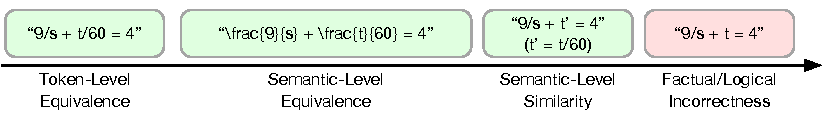
\includegraphics[width=0.9\textwidth]{figures/equiv_spectrum.pdf}
    \caption{The spectrum of approximations of one example reasoning step (equation 1 in Fig.~\ref{fig:toy_example}). \name{} can control the exactness of reasoning approximations by adjusting its acceptance threshold to navigate through the accuracy-latency tradeoff space (\S\ref{sec:acc_lat_tradeoff}).}
    \label{fig:equiv_spectrum}
\end{figure}






In this work, we show that reasoning workloads executed by LRMs exhibit unique opportunities for latency reduction due to their inherent tolerance to approximation--- setting them apart from traditional generation tasks in LLMs. We illustrate these properties using a representative example from the AIME dataset, selected for its clarity and ease of exposition.

\textbf{Intermediate steps are easier than end-to-end reasoning.} A key observation in LRM behavior is that reasoning difficulty is not uniform across the steps in a long chain-of-thought (CoT). As shown in Fig.~\ref{fig:toy_example}, while the overall task might be too challenging for a small model to solve end-to-end, only a few critical steps---such as problem analysis, decomposition through formulations or case analyses, and high-level planning---are critical to the overall reasoning progress. In contrast, many other steps are significantly easier.

This behavior is intentional by design: LRMs are often trained with reinforcement learning to generate CoTs that decompose complex problems into sequences of simpler, more tractable reasoning steps. These intermediate steps often include routine reasoning such as arithmetic calculations, case enumeration, or basic logical deductions---operators that are much easier to decode than synthesizing a full solution directly. This heterogeneity in step difficulty and importance creates an opportunity for lightweight models to handle a substantial portion of the reasoning process both efficiently and accurately.


\textbf{Reasoning progress depends on insights, not exact tokens.} Another key takeaway from our work is that the utility of a reasoning step lies in the semantic contribution it makes to the overall reasoning process, rather than the precise tokens it uses. Unlike tasks like translation in traditional LLM inference, where fidelity to exact combinations of tokens matters more, reasoning CoTs within LRM's thinking tokens care more about the information that advances the reasoning chain. 
As illustrated in Fig.~\ref{fig:equiv_spectrum}, a spectrum of valid phrasings often exists for a given step: semantically equivalent or similar expressions can convey the same insight and lead to the same downstream reasoning trajectory. This semantic flexibility is a key enabler for approximation-tolerant inference.

\textbf{Occasional mistakes can be corrected via self-reflection.} LRMs exhibit strong self-reflection capabilities, enabling them to recover from earlier reasoning errors. 
Even when an earlier step contains a factual or logical mistake, the model often revises its trajectory in subsequent steps, marked by tokens like ``Wait'' or ``Hmm''. Moreover, unlike LLM inference where {\em all} output tokens contribute to the final answer, in LRM inference, only the tokens generated {\em after} the thinking tokens determine the final outcome. Therefore, LRM inference can tolerate occasional mistakes during the reasoning phase, as the model can often identify and correct these mistakes during self-reflection. This inherent fault tolerance further underscores the viability and effectiveness of approximation-based acceleration.

In summary, compared to traditional LLM inference, LRM inference is inherently more tolerant of approximations that do not require token-level equivalence as long as the overall reasoning trajectory is preserved. This property is not limited to a single, linear CoT; rather, it extends naturally to more general inference-time compute scaling paradigms such as tree-based search strategies and other structured reasoning approaches.











